\documentclass{IEEEtran}

\hbadness=99999

% Packages
\usepackage{amsmath}
\usepackage{physics}
\usepackage[cmintegrals]{newtxmath}
\usepackage{graphicx}
\usepackage{xurl} % Makes urls better
\graphicspath{{./images}}

% Title Stuff
\title{Engineering breakdown voltage in a pn-junction diode}
\author{Chase A. Lotito, \textit{SIUC Undergraduate}}
\date{}

% Makes a header!
\markboth{ECE447 --- Semiconductor Devices --- Project 3, April 2024}{Shell \MakeLowercase{\text
it{et al.}}: A Novel Tin Can Link}

\begin{document}

\maketitle % Makes the title

% ABSTRACT
\begin{abstract}
    % [A brief statement on what you plan to do in this project.]
For this lab, the goal is to design a one-sided abrupt silicon pn-junction diode. This diode must have a breakdown voltage of at least 60V with a forward-bias current of 50mA when applying 0.625V. We know that the minority carrier lifetimes are \(\tau_0 = 2 \times 10^{-7} s\). The parameters to engineer are doping density and cross-sectional area.
\end{abstract}

\section*{Introduction}

For this pn-junction experiment, the \textit{PN Junction Lab} from nanoHUB.org was used \cite{sim}.

\section*{Part I: Analytical Design}

Since we are using silicon, \(\mu_n = 1350 ~ \text{cm}^2/\text{Vs}\) and \(\mu_p = 480 ~ \text{cm}^2/\text{Vs}\). And, I assume \(T=300 ~ \text{K}\).

Using the Shockley diode equation, we can back-solve for the reverse saturation current \(I_s\) in our diode:

\begin{align*}
    I_D &= I_s(e^{V_D/V_{th}} - 1) \\
    \implies I_s &= I_D(e^{V_D/V_{th}} - 1)^{-1} \\
    &= (0.050)(e^{0.625/0.0259} - 1)^{-1} \\
    &= 1.655 \times 10^{-12} ~ \text{A}
\end{align*}

We will use this quantity to match the reverse saturation current density \(J_s\) with doping densities and the device cross-sectional area.

A one-sided abrupt pn-junction will have either \(N_d >> N_a\) or vice-versa, so choosing the former, a \(n^+p\)-junction will be made. This means the doping density in the low-doped region of the one-sided junction \(N_B = N_a\). So, rearranging Equation (7.61) from the textbook:

\begin{align*}
    N_a &= \frac{\epsilon_s E^2_{crit}}{2qV_B} \\
        &= \frac{11.7 (8.854 \times 10^{-14}) (4\times10^{5})^2}{2(1.6\times10^{-19})(60)} \\
        & \boxed{N_a = 8.633\times10^{15} ~ \text{cm}^{-3}}
\end{align*}

Here, I assumed the critical electric field of silicon is \(4\times10^5 \text{V}/\text{cm}\).  

Then, since this is a \(n^+p\)-junction, I will just choose \(N_d\) to be some value larger than \(N_a\). I found graphically, when solving for the donor doping density using the equation for \(J_s\), the function was asymptotic, so it is somewhat arbitrary when choosing the donor doping density. However, it would not make sense to make this value arbitrarily large, since larger and larger doping densities will not affect the device performance after enough doping. The donor doping density I chose was:

\begin{equation*}
    \boxed{N_d = 1 \times 10^{19} ~\text{cm}^{-3}}
\end{equation*}

From here, we can calculate for the reverse saturation current density \(J_s\) using a form of Equation (8.27) from the textbook:

\begin{align*}
    J_s &= qn_i^2 \left( \frac{1}{N_a} \sqrt{\frac{D_n}{\tau_{n0}}} +  \frac{1}{N_d} \sqrt{\frac{D_p}{\tau_{p0}}}\right)
\end{align*}

Using the Einstein Relation, \(D/\mu = kT/q\), the equation can be rearranged:

% using \left. and \right. when breaking the equation to get rid of errors
\begin{align*}
    J_s &= n_i^2 \sqrt{qkT}  \left( \frac{1}{N_a} \sqrt{\frac{\mu_n}{\tau_{0}}} +  \frac{1}{N_d} \sqrt{\frac{\mu_p}{\tau_{0}}}\right) \\
        &= (1.5 \times 10^{10}) \sqrt{6.624\times10^{-40}} \left( \frac{1}{8.633\times10^{15}} \sqrt{\frac{1350}{2\times10^{-7}}} \right.\\ 
        & \left. + \frac{1}{1\times10^{19}} \sqrt{\frac{480}{2\times10^{-7}}} \right)
\end{align*}

\begin{equation*}
    \boxed{J_s = 5.514\times10^{-11} ~ \text{A}/\text{cm}^2}
\end{equation*}

Now, we can find the cross-sectional area \(A\), since \(I_s = AJ_s\).

\begin{align*}
    A &= I_s / J_s \\ 
      &= (1.655\times10^{-12}) / (5.514\times10^{-11}) \\
      & \boxed{A = 0.03 ~ \text{cm}^2}
\end{align*}

\section*{Part II: Verification using nanoHUB simulations}

In the \textit{PN Junction Lab} simulator, the input parameters are in Figure \ref{fig:inputs}, and the doping profile derived in Part I is shown in Figure \ref{fig:doping}.

\begin{figure}[!ht] 
    \centering
    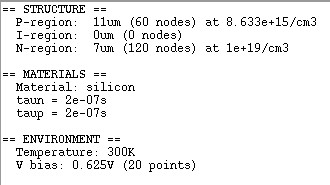
\includegraphics[width = 6cm]{inputs.jpg}
    \caption{Input Parameters in Simulator}
    \label{fig:inputs}
\end{figure}

\begin{figure}[!ht] 
    \centering
    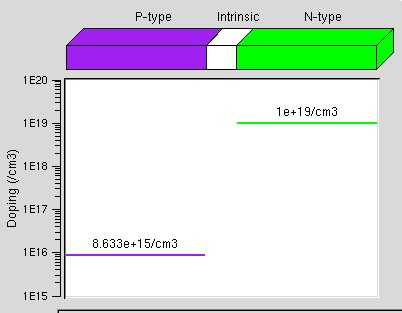
\includegraphics[width = 6cm]{doping.jpg}
    \caption{Doping Profile in Simulator}
    \label{fig:doping}
\end{figure}

Once the simulator have solved for the diode device characteristics, we see that for \(V_D = 0.625~\text{V}\) that \(J_D = 1.71751~\text{A} / \text{cm}^2 \). If we use the cross-sectional area from Part I, \(A = 0.03 ~ \text{cm}^2\), then we get the forward-bias diode current to be:

\begin{align*}
    I_D &= AJ_D \\
        &= (0.03)(1.71751) \\
        &= 0.0515 \\
        & \boxed{I_D = 51.5 ~ \text{mA}}
\end{align*}

\begin{figure}[!ht] 
    \centering
    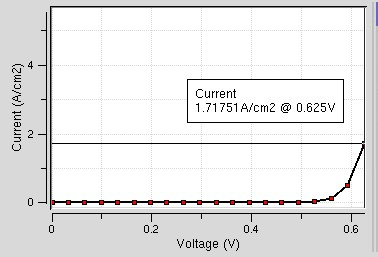
\includegraphics[width = 6cm]{current.jpg}
    \caption{IV-Characteristics in Simulator}
    \label{fig:current}
\end{figure}

\section*{Answers to Questions}

\textbf{What is the built-in potential in equilibrium, \(V_{bi}\)?}

\begin{align*}
    V_{bi} &= V_t \ln \left( \frac{N_a N_d}{n_i^2}  \right) \\
           &= (0.0259)\ln \left( \frac{(8.633\times10^{15})(1\times10^{19})}{(1.5\times10^{10})^2}  \right) \\ 
           &= 0.870 \\
           & \therefore ~ \boxed{V_{bi} = 0.870~\text{V}}
\end{align*}

\textbf{What is the maximum electric field, \(E_{max}\)?}

For the doping concentration in Silicon, \(E_{max} = 4\times10^5 ~ \text{V}/\text{cm}\).

\textbf{Is it possible to arbitrarily increase doping concentration?}

It is not practical to do so. Like I mentioned in Part I, \(J_s\) approaches a finite value as \(N_d \to \infty\). So, it is most efficient to choose the lowest possible doping density to achieve the current necessary, since it will be most cost-effective.

\textbf{Do you obtain the same forward-bias current from these two calculations? Why or why not?}

The currents are the same once I varied the p-type and n-type lengths in the simulator. In this case, the p-type region was \(11 \mu m\) and the n-type region was \(7 \mu m\). My guess is this changes the lengths over which the charge carriers diffuse in the diode, which is directly proportional to the current in the device.

\textbf{What happens to the I-V curve if the temperature is increased to 500K? Why?}

When re-simulating with \(T = 500\text{K}\), the I-V curve drastically increases in value. The new forward-bias diode current density for the same forward-bias voltage is \(J_D = 1176.59 ~ \text{A}/\text{cm}^2 \), which means the forward-bias diode current is \(I_D = 35.3 ~\text{A}\).

This is because the diode current is proportional to the intrinsic carrier density squared, and the intrinsic carrier density is exponentially dependent on temperature.

\begin{equation*}
    I_D \propto n_i^2 \propto e^{-E_g / kT}
\end{equation*}

\textbf{Using simulations, discuss what happens to the I-V curve if carrier lifetimes are increased by a factor of 100 (that is recombination is suppressed). }

Re-simulating the device with \(\tau_0 = 2 \times 10^{-5} ~\text{s}\), and \(T = 300\text{K}\), the forward-bias diode current density for the same forward-bias voltage is \(J_D = 1.62108 ~ \text{A}/\text{cm}^2 \), which means the forward-bias diode current is \(I_D = 48.6 ~\text{mA}\). Which is a slight decrease to our original current.

This is expected since the reverse saturation current is inversely dependent on the square roots of the minority carrier lifetimes. 

% REFERENCES!
\bibliographystyle{IEEEtran}
\bibliography{project3Bib.bib}

\end{document}
